%intro
%	db=entity, store data structured manner, little redundancy, allow user access, controlled concurrent access
%	useful: efficent data access and storage, concurrent, user access rights
%	describe scenario
%Queries & results
%	Just dump query txt and csv file into doc, give BRIEF desc
%Description
%	ER Model
%		Start with own, show errors, show given one, explain how fix errors
%	Relation Scheme
%		Entity types, own table with attribs as columns, apply primary/compund key constraint
%		Compound attribs, move into tabel as sperate arribs
%		Convert Staff subtypes into own tables, with one-to-one relationship with Staff table
%		Add tables for many-to-many relationships, one col is id of one relation and the other is the id of the other
%		Add relationship attribs to the relations which needs them
%		Add forgien key contraints for all relationships, including the resursive ones
%		Issue adding staff data sue toi recusive relationship, removed relationaship will adding data, then readd
%Conclusion & Reflections
%	Understand relationship attribs, integral for optimal design, could be worked around but not good design, not much effort as table for relationship existed
%	Failed fully understand combining multiple queries, allows for better query design, more processing done by DBMS the better

\documentclass[12pt]{article}
\usepackage{listings}
\usepackage{graphicx}

\author{Stuart Reilly}
\date{\today}
\title{CS1Q - Information Management Report}

\begin{document}
\maketitle

\newpage
\tableofcontents

\newpage

\section{Introduction}
A database is an entity which stores data in a structured manner while minimising redundancy, allowing user access and controlled concurrent access.
Before databases became popular, data was stored in files.
This did not allow for concurrent access of the data as the operating system would restrict the number of user with access to each file.
Also, there was no way to link the data, which caused redundancy.
Finally, each program would have to implement its own structure to its data, which causes potential inconsistencies between programs.
Databases solved these problems by allowing data to be linked through relationships and creating an abstraction between the physical layout of the data on disk and the program using it.
By providing the abstraction, any programs which use the data, can access the data in the same way.
In order to allow for concurrent access of the data, a database management system will lie between programs and the database.
The database management system will monitor and control who is trying to access the database, locking sections of the database while users use them.
This allows controlled concurrent access to the database, and allowing different user to be able to carry out a subset of the available database operations.
\\
\\
I was tasked to design and implement a database for the School of Computer Science which stores the details of students, courses, lecturer, assessments, tutorial groups and tutors.
It will store which student take which courses, the lecturers which teach each course and the assessments each student takes for their courses.
Also, which course has tutorial groups, which students are in each tutorial group and the tutor which leads each tutorial group.

\section{Queries And Results}
\subsection{Query 1}
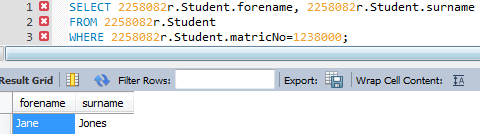
\includegraphics[width=\linewidth,height=3cm,keepaspectratio]{query/Query1}
\subsection{Query 2}
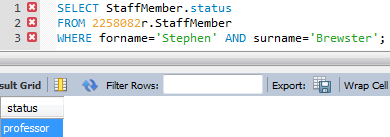
\includegraphics[width=\linewidth,height=3cm,keepaspectratio]{query/Query2}
\subsection{Query 3}
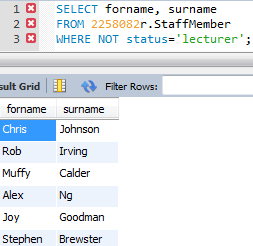
\includegraphics[width=\linewidth,height=5cm,keepaspectratio]{query/Query3}
\subsection{Query 4}
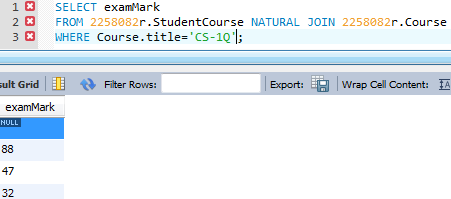
\includegraphics[width=\linewidth,height=4cm,keepaspectratio]{query/Query4}
\subsection{Query 5}
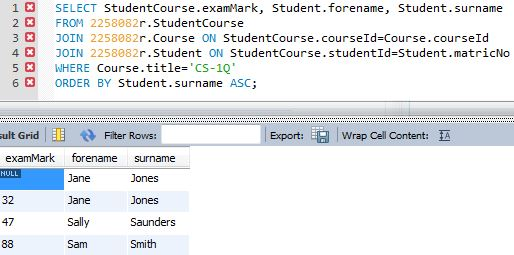
\includegraphics[width=\linewidth,height=4cm,keepaspectratio]{query/Query5}
\subsection{Query 6}
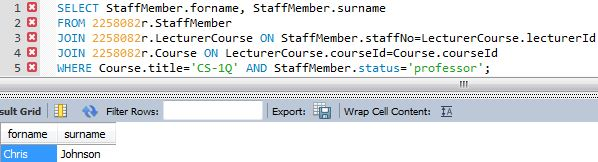
\includegraphics[width=\linewidth,height=3.5cm,keepaspectratio]{query/Query6}

\section{Description}
\subsection{Entity Relationship Diagram}
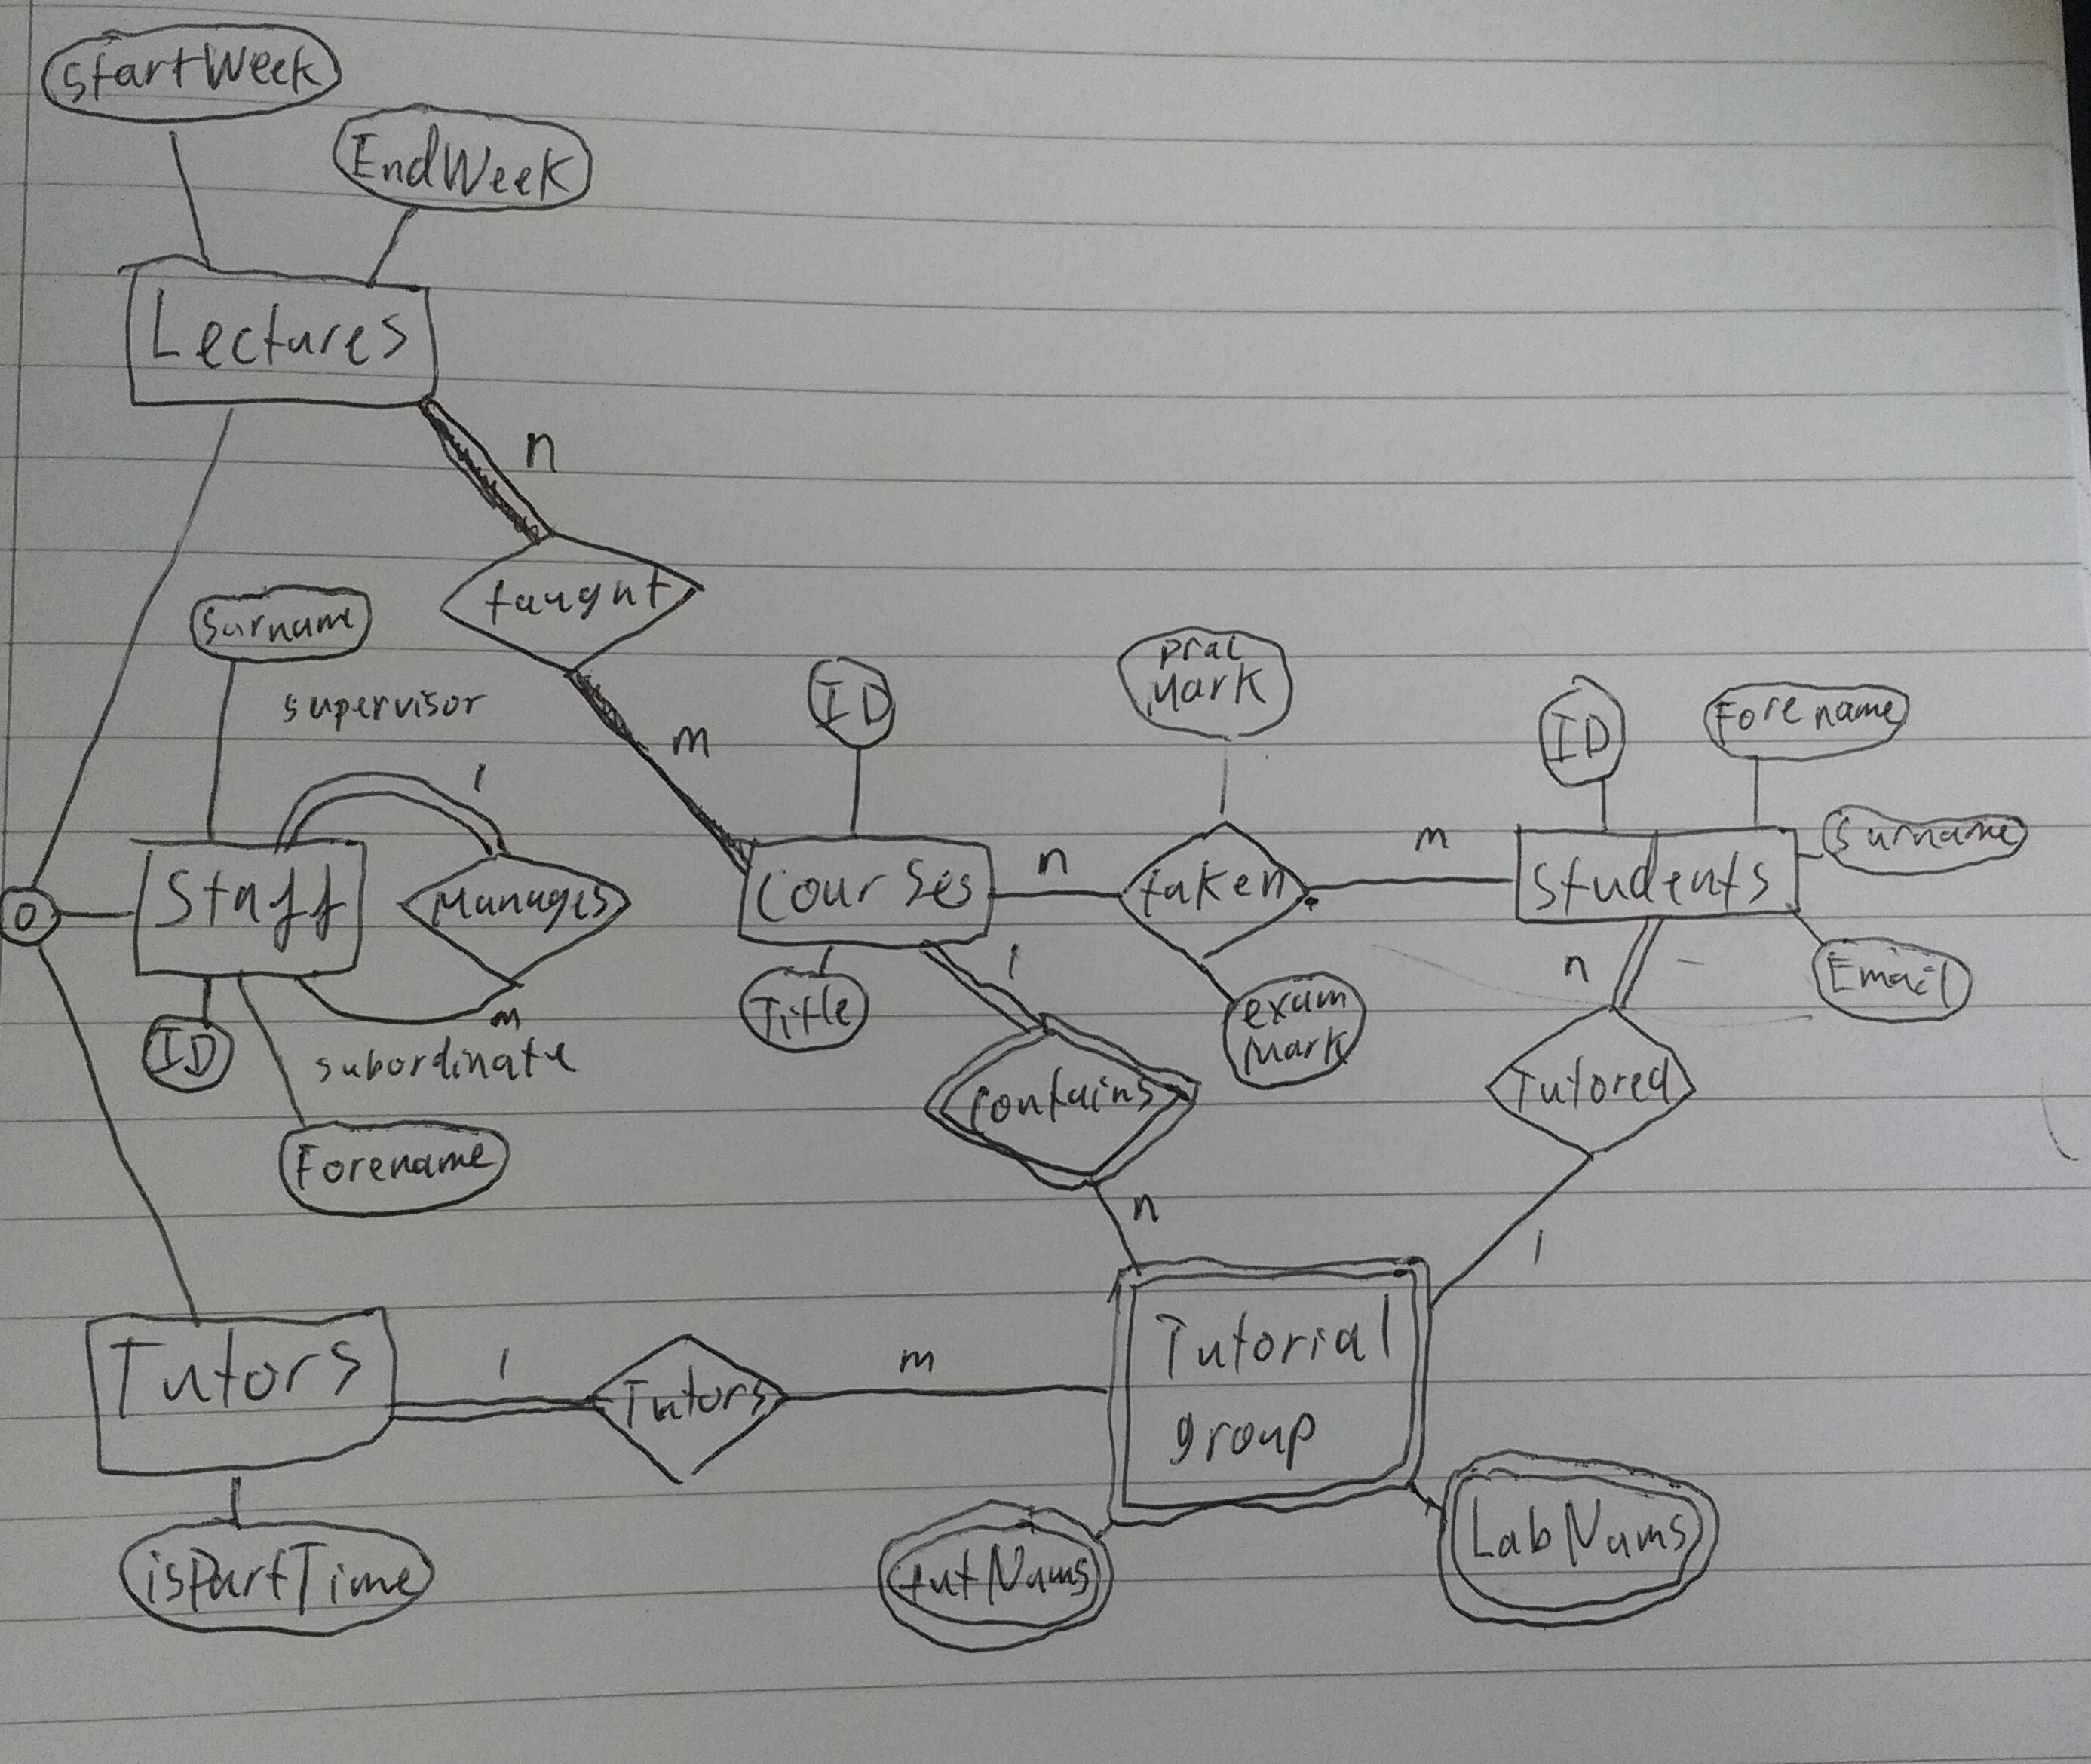
\includegraphics[width=\linewidth]{ER}
The above diagram is the initial entity relationship diagram I produced from the given brief, which had a number of flaws in its design.
Firstly, the Staff entity type is missing its Status attribute, which is required to determine the type of member of staff an entity is.
Next, the recursive relationship, to show which member of staff manages other member of staff, the supervisor side does not require total participation.
The same issue has occurred with both sides of the lecture-courses relationship the one side of the courses-tutorial group relationship and the many side of the students-tutorial group relationship.
Furthermore, the many side of the student-courses relationship does require total participation, because a course must have students.
Also, no primary keys have been defined for any relations.
Finally, the Tutorial Group entity should not be weak entity, as a weak entity means said entity cannot exist without a course, but a tutorial group can exist without being part of a course.
For example, there could be a tutorial group for helping students with their note taking skills.

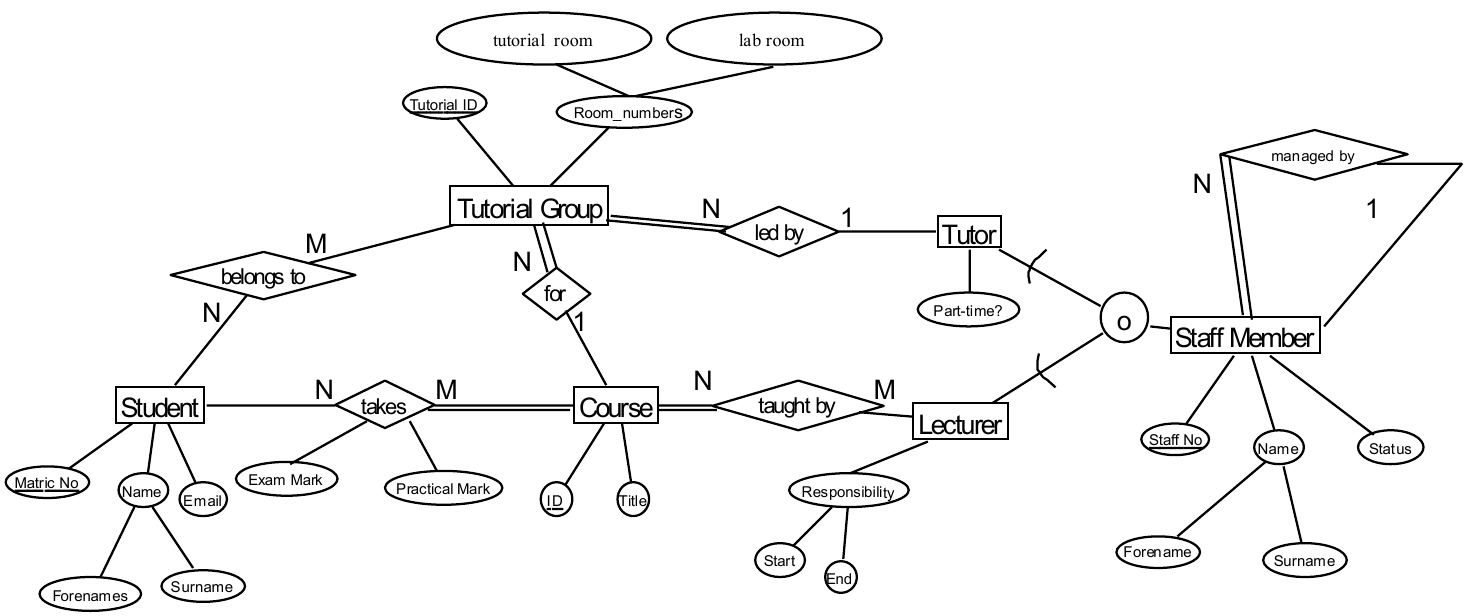
\includegraphics[width=\linewidth]{tut1_solution}
The above diagram is the final revision of my entity relationship diagram, where I addressed the previously stated issues.
The missing 'Status' attribute for the Staff Member entity type has been added and 'Staff No' has been assigned as Staff Member's primary key.
All entity types have been assigned a primary key and some attributes, such as Staff Member's Forename and Surname, have been combined into a composite attribute as they combine to form the data which would be stored if the composite attribute was one attribute.

\subsection{Relational Schema Design}
Using the above diagram, I designed and implemented a relational database schema, which involved converting the entity types and the many-to-many relationships into distinct relations.
A many-to-many relationship could be implemented without an intermediary relation, but it would cause a large amount of redundancy as each entry and its attributes will be repeated.
By adding an intermediary relation, with the primary keys of both relations involved as attributes, the relationship will be maintained without the added redundancy.
In order to design the Student-takes-Course relationship, the intermediary relation will be used to store the relationship attributes as its own attributes.
This allows a student to take exams for an undefined number of courses, whereas if the 'Exam Mark' and 'Practical Mark' were attributes on the Student relation, the maximum number of exams a student could take would have to be defined.
Most database management systems implementations do not natively support subtypes, which means the Staff Member inheritance hierarchy will have to be implemented manually.
In order to achieve similar functionality, a Staff Member relation will be created with both the Lecturer and Tutor relations having a one-to-one relationship with Staff Member.
Each entry in the Tutor and Lecturer relations will have a corresponding entry in the Staff Member relation.
Compound attributes are natively supported by most database management systems, so they have to be collapsed into individual attributes in their respective relation.
\\
\\
The following is the relational scheme I created from the above entity relationship diagram, where an underlined attribute is a primary or compound key and an italic attribute is a foreign key.\\\\
StaffMember(\underline{StaffNo:Int}, Forename:Varchar, Surname:Varchar, Status:Varchar, \textit{ManagedBy:Int})\\
Tutor(\underline{\textit{StaffNo:Int}}, ResponsabiltyStart:Int, ResponsibiltyEnd:Int)\\
Lecturer(\underline{\textit{StaffNo:Int}}, PartTime:Boolean)\\
Course(\underline{ID:Int}, Title:Varchar)\\
TutorialGroup(\underline{TutorialId:Int}, TutorialRoom:Varchar, LabRoom:Varchar, \textit{Tutor:Int}, \textit{Course:Int})\\
Student(\underline{MatricNo:Varchar}, Forename:Varchar, Surname:Varchar, Email:Varchar)\\
LecturerCourse(\underline{\textit{CourseId:Int}, \textit{LecturerId:Int}})\\
StudentCourse(\underline{\textit{StudentId:Int}, \textit{CourseId:Int}}, ExamMark:Int, PracticalMark:Int)\\
StudentTutorial(\underline{\textit{StudentId:Int}, \textit{TutorialGroupId:Int}})\\

\subsection{Populating the Database}
A database without any data is not very useful.
In order to populate the database efficiently, I used MySQL Workbench's built in CSV loading functionality.
This produces SQL similar to the following:
\begin{lstlisting}
LOAD DATA INFILE 'data.csv' INTO TABLE dbname.table;
\end{lstlisting}
Using this method exposed an issue with the design of the Staff Member relation.
When adding a new staff member, it must have a 'ManagedBy' attribute, but as the table is empty initially, there is no member of staff to reference when adding the initial member of staff.
This was solved by temporarily removed the foreign key constraint until the initial member's of staff were added.

\subsection{Querying the Database}
In order to access the data, one must query the database using SQL.
SQL is a declarative language, in which you define what data is needed and what form it should be in, the database management system converts that into relational algebra for the database engine to execute.
In order to from a SQL query, I had to find what data I needed and what form it had to be in from the task.
For example, if I was asked to find the names of all the professors, the data is the Staff Member data, filtered to only those who's status is 'professor' and the form is their forename and surname.
Hence, I would use the following SQL to retrieve the data:
\\\\
SELECT Forename,Surname FROM StaffMember WHERE Status=="professor";
\\\\
This is an example of a basic query.
It only references one table and has a simple condition.
\\\\
Another type of query is an Equi-Join query, where the data required is in more than one relation.
An example would be: Find all the tutorial rooms for CS1Q.
In order to get the required data, I need to join the Course relation and the Tutorial relation, using the foreign key in the Tutorial relation, then filtering by the course name, and projecting only the tutorial room attribute of the Tutorial relation.
This would be done using the following SQL:
\\\\
SELECT TutorialGroup.tutorialRoom FROM TutorialRoom, Course WHERE TutorialRoom.course==Course.courseId AND Course.title=="CS1Q";
\\
\section{Conclusion and Reflections}
During this project, I gained an understanding for relationship attributes.
Although, they are not required to design a database, they allow for an optimised design and reduced redundancy.
If they were not used in the design of my database, each entry on the Student relation would have to be repeated twice per course the student had enrolled in.
By using relationship attributes, this redundancy is removed and it allows for better querying of student's results as rather than processing a large Student relation, a relatively small relation can be processed, reducing the overall cost of the query.
I also began working with combining multiple queries to form a single result during this project.
Sadly, I was not able to fully grasp the concept as I could not quite understand fully how to combine the results of the sub-queries.
If I understood combing multiple queries, I could further optimise querying the database, because it reduces the amount of processing of the data the program accessing the database has to do and allocating the processing to the database, which is more optimised to carry out such tasks.

\end{document}
